Our model is easily amenable to a distributed implementation using asynchronous distributed stochastic gradient descent~\citet{Chilimbi14}. % \citep{Chilimbi14, MartinAbadi15}. 
Our distributed setting, % \footnote{Currently, we use a CPU-only compute cluster.}
based on TensorFlow, includes one or more \emph{Parameter servers} (\name{ps}), and a number of \emph{Workers}. 
The latter proceed asynchronously using randomly selected batches of data: they fetch fresh model parameters from the \name{ps}, compute the gradients of the lower bound with respect to these parameters, and push those gradients back to the \name{ps}, which update the model accordingly. 
Given that workers compute gradients and send updates to \name{ps} asynchronously, the  discrepancy between the model used to compute gradients and the model actually updated can degrade training quality. 
This is exacerbated by a large number of asynchronous workers, as noted in~\citet{Chen16}.

We focus our experiments on the MNIST dataset, and study how training time and error rates evolve with the number of workers introduced in our system. 
The parameters for the model are identical to those reported for the previous experiments.

\pgfplotsset{label style={font=\Large}, title style={font=\Large}}
%\pgfplotsset{label style={font=\Large}, title style={font=\Large}}

\begin{figure}[ht]
\begin{center}
%% \begin{tabular}{c}
 {\scriptsize \bf  MNIST} \\
%% {\small MNIST-8M}\\
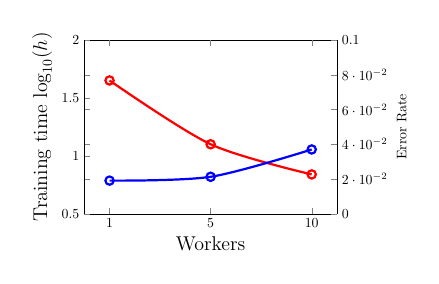
\begin{tikzpicture}[scale=0.5]
\begin{axis}[
    xmin=0, xmax=4,
  axis y line*=left,
	width=8cm, height=6cm,
  ylabel={Training time $\log_{10}(h)$},
  ymin=0.5, ymax=2,
  xlabel=Workers,
  xmin = 0.75, xmax = 3.25,
  xtick= {1,2,3},
  xticklabels={},
  extra x ticks={1,2,3},
  extra x tick style={xticklabels={1,5,10}}
  %xticklabels={0,1,5,10,15},
]
\addplot[smooth, mark=o, mark size=3pt, red, ultra thick]
coordinates{
    (1,1.65)
    (2,1.10)
    (3,0.84)
}; \label{plot_one}
%\addlegendentry{plot 1}
\end{axis}

\begin{axis}[
	width=8cm, height=6cm,
  ylabel={Error Rate},
  axis x line=none,
  xmin = 0.75, xmax = 3.25,
  ymin=0, ymax=0.1,
  ylabel near ticks, yticklabel pos=right
%% axis y line*=right
]
\addplot[smooth, mark=o, mark size=3pt, blue, ultra thick]
  coordinates{
    (1,0.0191)
    (2,0.0213)
    (3,0.037)
}; \label{plot_two}
%\addlegendimage{/pgfplots/refstyle=plot_one}\addlegendentry{plot 1}
%\addlegendimage{/pgfplots/refstyle=plot_two}\addlegendentry{plot 2}
\end{axis} 
\end{tikzpicture} 
%% &
%% \begin{tikzpicture}[scale=0.32]
%% \pgfplotsset{
%%     scale only axis,
%%     xmin=0, xmax=4
%% }

%% \begin{axis}[
%%   axis y line*=left,
%%   ylabel={Training time},
%%   ymin=6, ymax=17,
%%   xlabel=Workers,
%%   xmin = 0.75, xmax = 3.25,
%%   xtick= {1,2,3},
%%   xticklabels={},
%%   extra x ticks={1,2,3},
%%   extra x tick style={xticklabels={1,5,10}}
%%   %xticklabels={0,1,5,10,15},
%% ]
%% \addplot[smooth, mark=o, mark size=3pt, red, ultra thick]
%%   coordinates{
%%     (1,16)
%%     (2,12.6)
%%     (3,8)
%% }; \label{plot_one}
%% %\addlegendentry{plot 1}
%% \end{axis}

%% \begin{axis}[
%%   axis y line*=right,
%%   ylabel={Error Rate},
%%   axis x line=none,
%%   xmin = 0.75, xmax = 3.25,
%%   ymin=0, ymax=0.22
%% ]
%% \addplot[smooth, mark=o, mark size=3pt, blue, ultra thick]
%%   coordinates{
%%     (1,0.01)
%%     (2,0.04)
%%     (3,0.15)
%% }; \label{plot_two}
%% %\addlegendimage{/pgfplots/refstyle=plot_one}\addlegendentry{plot 1}
%% %\addlegendimage{/pgfplots/refstyle=plot_two}\addlegendentry{plot 2}
%% \end{axis} 
%% \end{tikzpicture}\\
%% \multicolumn{1}{c}{
\includegraphics[width=150pt]{figures/legend_async.pdf}
%% }
%% \end{tabular}
\end{center}
\caption{Comparison of training time and error rate for asynchronous \name{dgp-rbf} with 1, 5 and 10 workers.}
\label{fig:async}
\end{figure}


We report the results in Figure~\ref{fig:async}, and as expected, the training time decreases in proportion to the number of workers, albeit sub-linearly.
On the other hand, the increasing error rate confirms our intuition that imprecise updates of the gradients negatively impact the optimization procedure. 
The work in~\citet{Chen16} corroborates our findings, and motivates efforts in the direction of alleviating this issue.
